\section{Beyond the Scan Chain}
\label{sec:beyond_scanchain}
The biggest limitation of the scan chain based architecture was the IO bandwidth and latency.
A new architecture was needed for TinyTapout 4, so proposals were gathered from the community.
An online video call was held and the 10 proposals discussed.
The winning design was a fairly straightforward multiplexer design shown in Fig.~\ref{fig:multiplexer_design}.

\begin{figure}[!t]
\centering
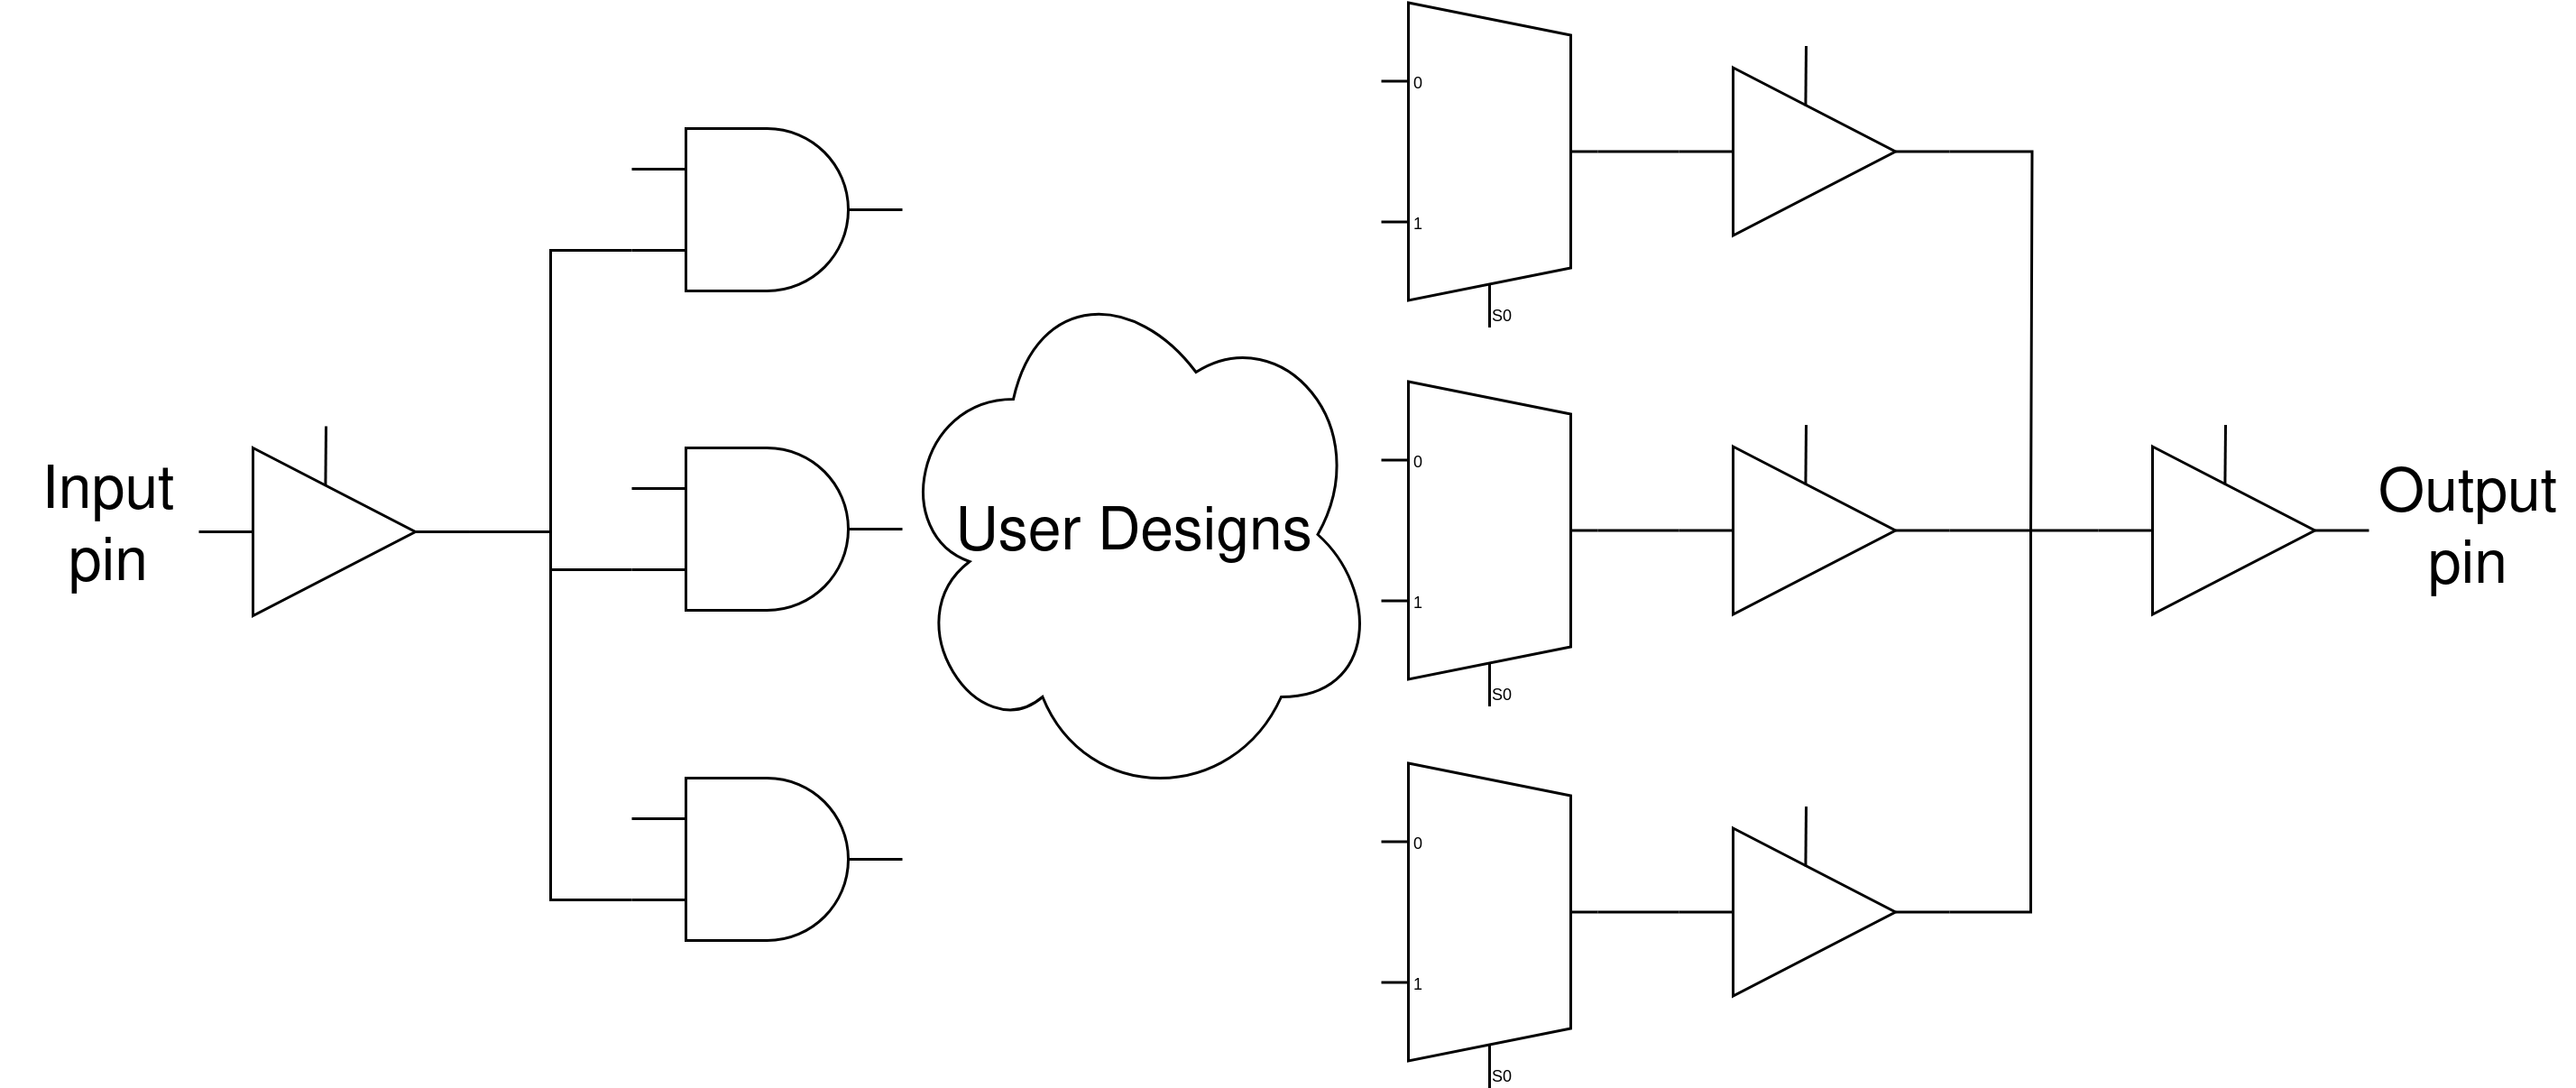
\includegraphics[width=\columnwidth]{./Figs/mux architecture.png}
\caption{Simplified diagram of the multiplexer architecture.}
\label{fig:multiplexer_design}
\end{figure}

The physical layout (shown in Fig.~\ref{fig:TT03_5_test_design}) consists of a central controller connected up and down to two vertical spines.
Twenty-four horizontal muxes connect to the spine with each supporting 16 designs.
This allows up to 384 separate single tile designs.
Multiple tile designs were also enabled, allowing a maximum project size of $8 \times 2$ tiles or $1359 \times \qty{225}{\um\squared}$---around \num{20000} logic cells. Table~\ref{tab:comparison_TT03_TT04} shows the key differences between TT03 and TT04.

\begin{figure}[!t]
\centering
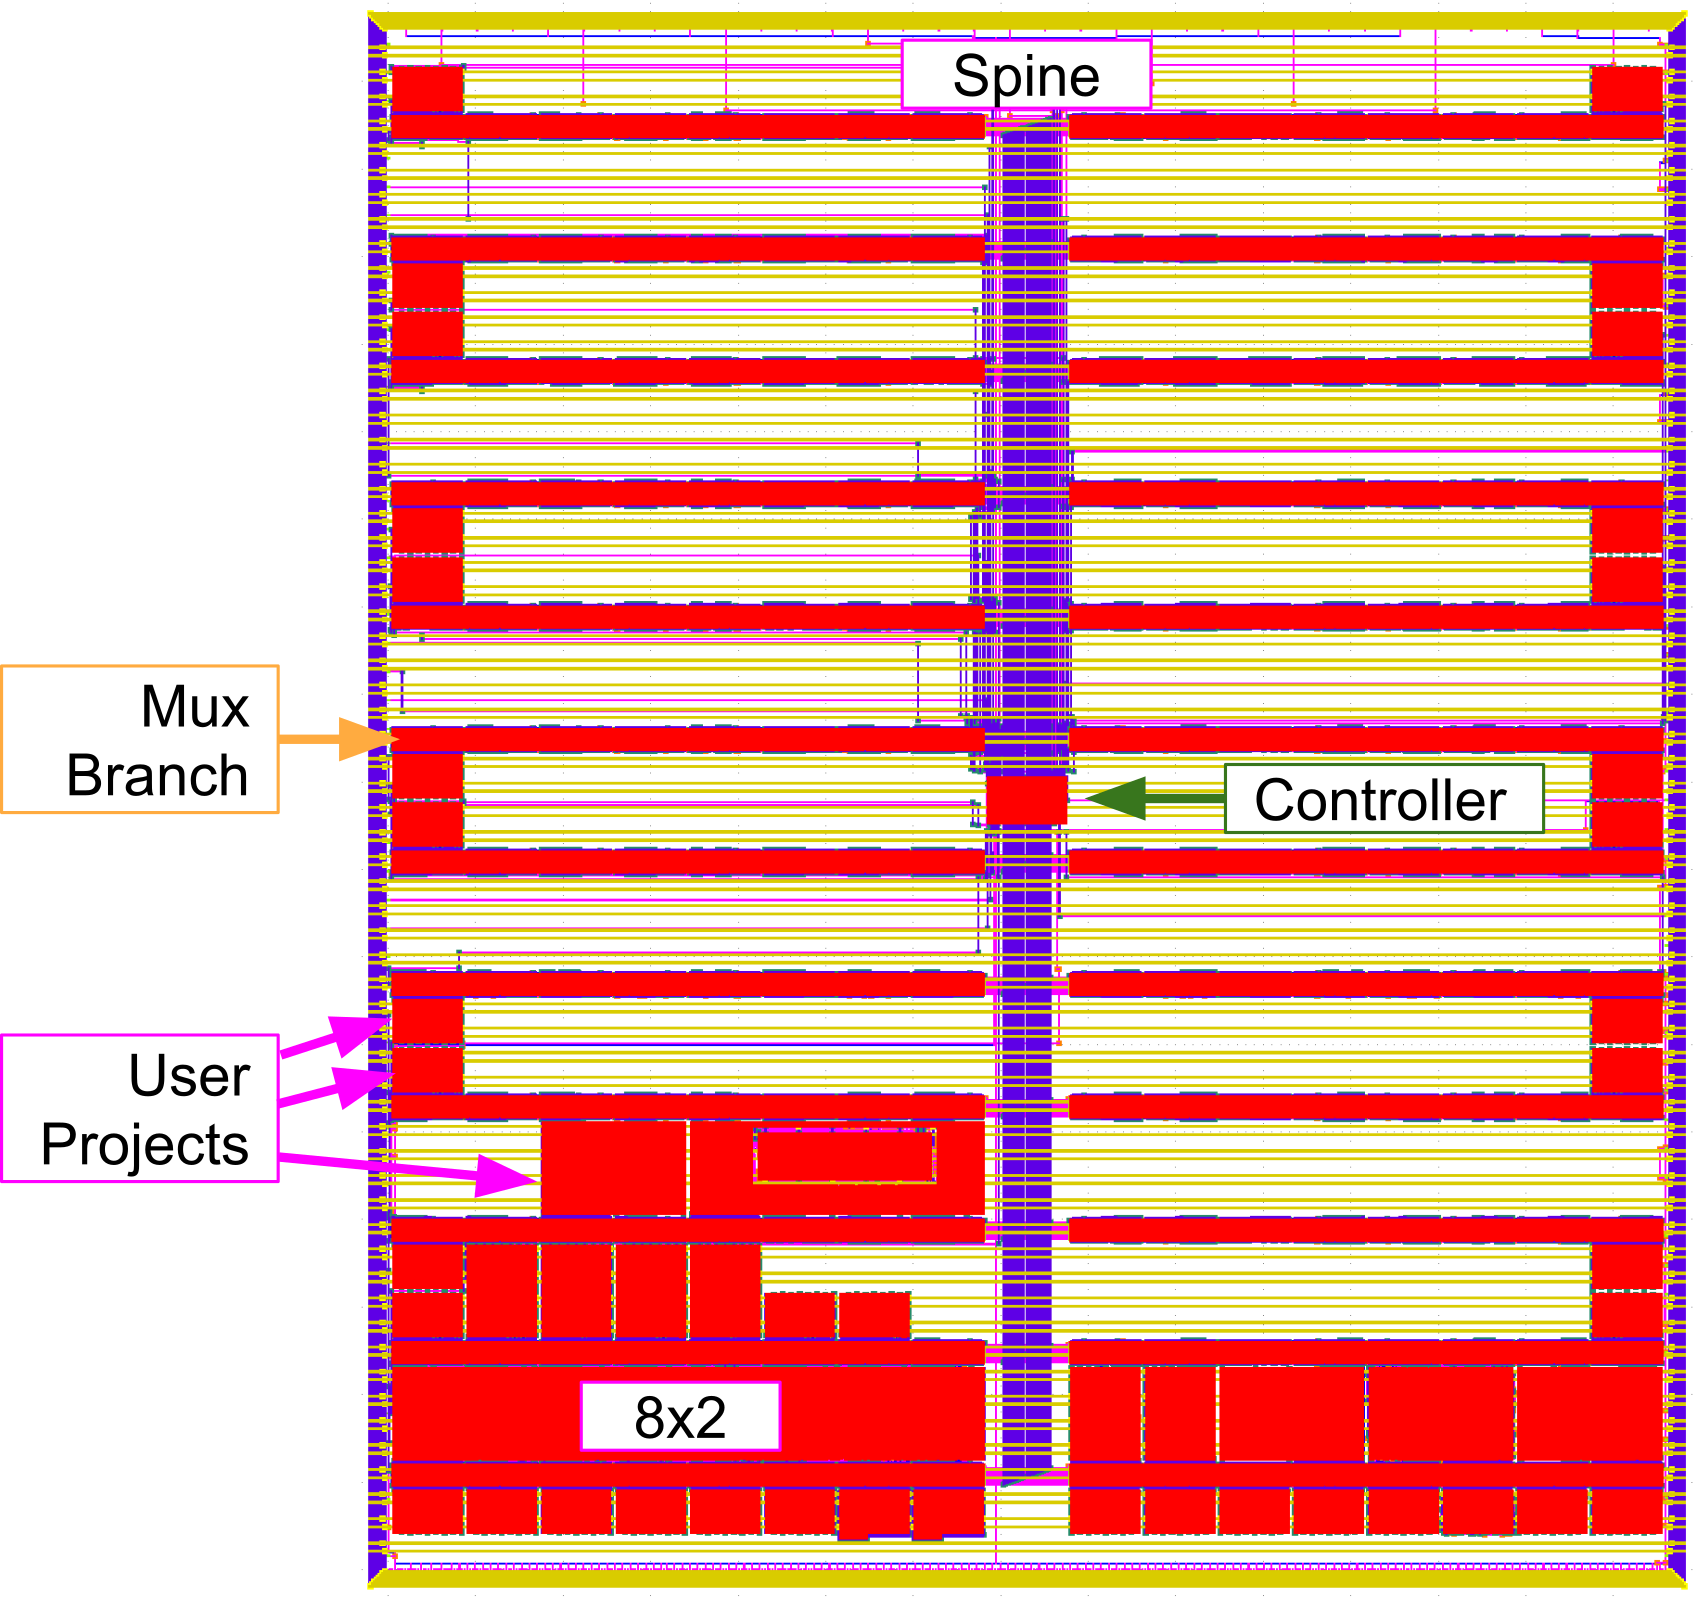
\includegraphics[width=\columnwidth]{./Figs/tt3p5 layout.png}
\caption{The TT03.5 test design.}
\label{fig:TT03_5_test_design}
\end{figure}

Another major limitation of TT01 to TT03 was the small number of IO.
The scan controller used 9 GPIOs to select the currently active design, which, while simplifying the demo board, wasted valuable pins.
With TT04, the parallel design selection was dropped in favor of a serial protocol.
The extra pins were then used as bidirectional pins, giving each design clock, reset, and 24 IO.

\begin{table}[!t]
\centering
\caption{Comparison between TT03 and TT04}
\label{tab:comparison_TT03_TT04}
\begin{tabular}{@{}lcc@{}}
\toprule
Parameters & TT03 & TT04 \\
\midrule
Max clock speed & \qty{12.5}{\kHz} & \qty{50}{\MHz} \\
Max design size & $150 \times \qty{170}{\um\squared}$ & $1359 \times \qty{225}{\um\squared}$ \\
Input pins & 8 & 10 \\
Output pins & 8 & 8 \\
Bidirectional I/O pins & None & 8 \\
Custom GDS file & \xmark & \checkmark \\
\bottomrule
\end{tabular}
\end{table}

An invite-only experimental shuttle~\cite{tinytapeout03p5} was submitted with 32 designs to Efabless chipIgnite 2306C.
Two of the designs included a power gate as a stepping stone to supporting analog and mixed-signal designs.
